\documentclass[11pt,a4paper]{article}
\usepackage[margin=2.5cm]{geometry}
\usepackage{graphicx,booktabs,amsmath,float,caption,fancyhdr,xcolor,enumitem,tabularx}
\usepackage[hidelinks]{hyperref}
\captionsetup{font=small,labelfont=bf}
\setlist{itemsep=2pt,topsep=4pt}
\pagestyle{fancy}\fancyhf{}
\lhead{QuakeWatch}\rhead{Big Data Management | Project Report}
\cfoot{\small Anurag, Kushagra, Kshitij, Vibhor \quad|\quad \thepage}
\renewcommand{\headrulewidth}{0.3pt}
\newcommand{\fig}[3]{\begin{figure}[H]\centering\includegraphics[width=#2\linewidth,height=0.42\textheight,keepaspectratio]{figures/#1}\caption{#3}\end{figure}}
\newcommand{\repo}{\url{https://github.com/vibhor-5/quakewatch-bdm}}

\begin{document}
\begin{titlepage}
\centering\vspace*{1.2cm}
{\large BIG DATA MANAGEMENT}\\[1.2cm]
{\Huge\bfseries QuakeWatch}\\[0.4cm]
{\Large Spatial and Temporal Analysis\\of Global Earthquakes}\\[0.6cm]
{\large An analysis of USGS ComCat records using\\MongoDB, Python, React and a BI dashboard}\\[1.6cm]
A project report submitted for the course\\\textbf{Big Data Management (Semester VII)}\\[1.2cm]
Submitted by\\[0.3cm]
\begin{tabular}{lll}
Anurag & Roll No.: 2023IMG-008 \\
Kushagra & Roll No.: 2023IMG-030 \\
Kshitij & Roll No.: 2023IMG-029 \\
Vibhor & Roll No.: 2023IMG-054 \\
\end{tabular}\\[0.8cm]
IMG (Integrated B.Tech + MBA)\\[0.8cm]
{\bfseries ATAL BIHARI VAJPAYEE\\INDIAN INSTITUTE OF INFORMATION TECHNOLOGY\\AND MANAGEMENT GWALIOR}\\
Gwalior, India\\[0.6cm]
November 2026\\[1cm]
{\small Source code: \repo}
\end{titlepage}

\section*{Abstract}
QuakeWatch examines when and where earthquakes are recorded around the world, and how the share of strong events (magnitude 5.0 or above) varies with depth, magnitude type, contributing network and region. The project uses the U.S. Geological Survey (USGS) ComCat catalogue of earthquakes with magnitude 2.5 or above for 2024 and 2025. Python prepares the records for three MongoDB collections holding 55,152 documents. A Flask API supplies a React web application, and a separate export pipeline prepares six tables for a business-intelligence dashboard.

The catalogue contains 53,952 tectonic earthquakes, of which 3,636 are strong, giving a strong share of 6.74\%. The largest event, a magnitude 8.8 earthquake off Kamchatka on 29 July 2025, produced about 82.6\% of all seismic energy radiated in 2025 and a burst of aftershocks that doubled the July event count (4,157 against 2,043 a year earlier). Strong share varies enormously with magnitude type (79.3\% for moment magnitude \texttt{mww}, 0.07\% for local magnitude \texttt{ml}); we show this reflects \emph{how events are reported} and not physical differences. Hourly and weekday counts are essentially flat, as expected for a natural process. A five-run local benchmark records a median of 0~ms for indexed queries against 12--41~ms for collection scans on 53,952 documents, with 25 to 54,000 times fewer documents examined. Unlike the spatial query in many first attempts, a bounded \texttt{\$geoWithin} query uses the 2dsphere index effectively here.

\medskip\noindent\textbf{Keywords:} USGS ComCat, earthquakes, MongoDB, spatial aggregation, magnitude--frequency, BI dashboard.

\tableofcontents
\newpage

\section{Introduction}
Earthquake catalogues combine a physical process (stress release along faults) with a measurement process (seismometer networks, magnitude scales, review procedures). Analysing them demands care about what a number actually counts. The purpose of QuakeWatch is to turn a public catalogue into a usable analytical system: national and regional summaries, time patterns, geographic exploration, condition-based comparison of strong-event share, and inspection of individual events.

\subsection{Questions addressed}
\begin{enumerate}
\item How does earthquake volume vary by month, hour of day and day of week?
\item Which depth classes, magnitude types, networks and regions have a higher share of strong events?
\item How do spatial concentrations of events differ from concentrations of strong events?
\item How much work do MongoDB indexes save for representative queries, including a geospatial one?
\item How can the same prepared data support both a web application and a BI dashboard?
\end{enumerate}

\fig{architecture.png}{0.95}{Implemented data flow. The web application reads MongoDB through Flask; the dashboard consumes CSV tables exported from the same prepared data. This is an architecture diagram, not a screenshot.}

\subsection{Scope}
The project demonstrates ingestion, indexing, aggregation and presentation on one local MongoDB instance. It does not demonstrate distributed processing, a production deployment, seismic hazard modelling or earthquake prediction.

\section{Data and Preparation}
\subsection{Source and coverage}
The source is the USGS Earthquake Hazards Program ComCat catalogue, accessed through its FDSN event web service.\cite{usgs} We requested all events with magnitude 2.5 or above for each calendar month of 2024 and 2025 as CSV. The catalogue merges contributions from many networks, so completeness differs by region: the global network is complete to roughly magnitude 4.5, while US regional networks also report smaller events.

\begin{table}[H]\centering
\caption{Imported records, checked against MongoDB and the saved import report.}
\begin{tabular}{llr}\toprule
Collection & Content & Documents\\\midrule
\texttt{earthquakes} & one document per earthquake & 53,952\\
\texttt{daily\_summary} & one document per date (2024--2025) & 731\\
\texttt{region\_summary} & one document per region and year & 469\\\midrule
Total & & 55,152\\\bottomrule
\end{tabular}
\end{table}
The raw download holds 54,394 rows (24 monthly files, no duplicate event identifiers). The 442 rows whose event type is not ``earthquake'' (415 mining explosions, 9 ice quakes and 18 others) were excluded so that the analysis concerns tectonic events. No coordinates were invalid and no magnitude or depth was missing among the retained events.

\subsection{Preparation pipeline}
\begin{enumerate}
\item \textbf{Download and provenance.} \texttt{download\_data.py} saves each CSV and a manifest with the request URL, timestamp, size, row count and SHA-256 hash.
\item \textbf{Time fields.} Timestamps are converted to UTC; year, month, hour, weekday and date are derived for aggregation.
\item \textbf{Classes.} Depth is binned as Shallow ($<70$~km), Intermediate (70--300~km) and Deep ($>300$~km). Magnitude is binned as Minor (2.5--3.9), Light (4.0--4.9), Moderate (5.0--5.9), Strong (6.0--6.9) and Major (7.0+). An event is \emph{strong} if $M \ge 5.0$.
\item \textbf{Regions.} The region is the text after the last comma of the USGS \texttt{place} string; US state names are merged into ``United States''. This gives 273 distinct regions and is a heuristic, not an official gazetteer.
\item \textbf{Grid identifier.} Coordinates are floored into $2^\circ\times2^\circ$ cells and the cell centre forms a grouping key. There are 2,246 non-empty cells. Valid points are stored as GeoJSON (longitude, latitude) for the 2dsphere index.
\item \textbf{Energy.} Radiated energy is estimated with the Gutenberg--Richter relation $\log_{10}E = 1.5M + 4.8$ (joules).\cite{gr56}
\end{enumerate}

\subsection{Record structure}
Each event is identified by the USGS event id, which is used as the MongoDB \texttt{\_id}. The two summary collections are derived from it and are rebuilt on every import.

\section{Analytical Method}
\subsection{Units and denominators}
For a subset $X$ let $n_X$ be all catalogued events and $s_X$ those with $M\ge5.0$. Define
\begin{equation}
p_X=\frac{s_X}{n_X},\qquad \text{strong share}(X)=100\,p_X .
\end{equation}
The full 2024--2025 baseline is $p_B = 3{,}636/53{,}952 = 0.0674$. To compare a subset with this baseline we use a share ratio and an odds ratio:
\begin{equation}
R_X=\frac{p_X}{p_B},\qquad \mathrm{OR}_X=\frac{p_X/(1-p_X)}{p_B/(1-p_B)} .
\end{equation}
These are ratios of proportions among catalogued events. They do not measure seismic hazard, and because the baseline contains the subset, the comparison is descriptive.

\subsection{Support and interpretation}
Ranked combinations retain groups of at least 100 events; the application's map default is 25 events per cell. No confidence intervals, completeness corrections, causal estimates or out-of-sample predictions are claimed.

\section{Results and Analysis}
\subsection{Annual totals and magnitude distribution}
\begin{table}[H]\centering
\caption{Annual event counts and strong share.}
\begin{tabular}{lrrrr}\toprule
Period & Events & Strong ($M\ge5$) & Share & Largest\\\midrule
2024 & 24,954 & 1,507 & 6.04\% & M7.5\\
2025 & 28,998 & 2,129 & 7.34\% & M8.8\\
Combined & 53,952 & 3,636 & 6.74\% & M8.8\\\bottomrule
\end{tabular}
\end{table}
2025 records 4,044 more events (+16.2\%). Events of magnitude 6 or above rise from 99 to 145 and of magnitude 7 or above from 10 to 16. The magnitude classes contain 21,475 Minor, 28,841 Light, 3,392 Moderate, 218 Strong and 26 Major events. The cumulative count falls close to ten-fold per magnitude unit (Figure~\ref{fig:gr}); a maximum-likelihood estimate\cite{aki65} for $M\ge4.5$ ($n=14{,}956$) gives $b\approx1.23$, in the usual range for global catalogues, although a single combined catalogue with mixed completeness makes this only indicative.

\fig{gutenberg.png}{0.6}{Cumulative number of events at or above each magnitude threshold (log scale). The dotted line marks $M4.5$, the approximate global completeness limit.\label{fig:gr}}

\subsection{The July 2025 Kamchatka sequence}
Figure~\ref{fig:monthly} shows that monthly counts are steady near 2,000--2,300 until July 2025, when they jump to 4,157 (July 2024: 2,043) and remain elevated in August (3,055). The cause is the M8.8 earthquake at 23:24 UTC on 29 July 2025 off the Kamchatka Peninsula (event \texttt{us6000qw60}, depth 35~km). Within two weeks of the mainshock, the rectangle $48$--$54^\circ$N, $156$--$164^\circ$E holds 1,731 events, 263 of them strong. Removing that window lowers the 2025 strong share from 7.34\% to 6.84\% (27,267 events), so most, but not all, of the rise from 2024's 6.04\% comes from this one sequence.

Energy is even more concentrated: summing $10^{1.5M+4.8}$ gives about 0.084~EJ in 2024 and 1.21~EJ in 2025, a factor of 14, and the single M8.8 event accounts for 82.6\% of the 2025 total. Event counts and radiated energy tell very different stories.

\fig{monthly.png}{0.8}{Monthly earthquake counts. The July--August 2025 rise follows the M8.8 Kamchatka earthquake and its aftershocks.\label{fig:monthly}}

\subsection{Depth class}
\begin{table}[H]\centering
\caption{Strong share by depth class.}
\begin{tabular}{lrrr}\toprule
Depth class & Events & Strong & Share\\\midrule
Shallow ($<70$ km) & 42,131 & 3,043 & 7.22\%\\
Intermediate (70--300 km) & 9,473 & 478 & 5.05\%\\
Deep ($>300$ km) & 2,348 & 115 & 4.90\%\\\bottomrule
\end{tabular}
\end{table}
Shallow events have the highest strong share, but the differences are modest and sensitive to where networks report small events; deep events occur mainly beneath subduction zones that are well covered by global rather than dense regional networks.

\subsection{Magnitude type, network and review status}
Strong share depends dramatically on how the magnitude was computed (Table~\ref{tab:magtype}, Figure~\ref{fig:share}).

\begin{table}[H]\centering
\caption{Strong share by magnitude type (types with at least 100 events).\label{tab:magtype}}
\begin{tabular}{lrrr}\toprule
Magnitude type & Events & Strong & Share\\\midrule
\texttt{mww} (moment, W-phase) & 2,648 & 2,099 & 79.27\%\\
\texttt{mb} (body wave) & 29,391 & 1,489 & 5.07\%\\
\texttt{mw}, \texttt{mwr} (moment) & 1,389 & 26 & 1.87\%\\
\texttt{ml} (local) & 16,155 & 12 & 0.07\%\\
\texttt{md} (duration) & 4,192 & 0 & 0.00\%\\
\texttt{mb\_lg} & 161 & 0 & 0.00\%\\\bottomrule
\end{tabular}
\end{table}
These differences are not physical. The USGS computes W-phase moment magnitudes (\texttt{mww}) for larger events; local and duration magnitudes are used by regional networks for small ones. Likewise the \texttt{us} network contributes 41,778 events with a strong share of 8.64\%, while Alaska (\texttt{ak}, 3,478 events) has 0.35\% and Puerto Rico (\texttt{pr}, 3,052) 0.16\%. All 644 events with status \emph{automatic} (not yet reviewed) are below $M5$; the 53,308 reviewed events have 6.82\%.

\fig{share_conditions.png}{0.95}{Strong share by depth class and magnitude type. The dashed line marks the 6.74\% baseline.\label{fig:share}}

\subsection{Combinations of conditions}
Among depth-class $\times$ magnitude-type groups with at least 100 events, shallow \texttt{mww} events have a strong share of 78.91\% (2,134 events; share ratio 11.71, odds ratio 51.79) and intermediate \texttt{mww} events 77.08\% (432 events; 11.44 and 46.55). At the other extreme, shallow \texttt{ml} events (14,237) have 0.08\%. A like-for-like comparison with the same magnitude type is more informative: shallow \texttt{mb} events have a strong share of 6.39\% (20,549 events) against 1.46\% for deep \texttt{mb} events (2,266), a ratio of 4.38. These figures identify subsets for closer investigation; they do not rank regions by hazard.

\subsection{Time of day and weekday}
\fig{hourly.png}{0.75}{Events by hour of day (UTC), both years combined.}
Counts range only from 2,115 (19:00 UTC) to 2,431 (04:00 UTC) per hour, and weekday counts from 7,552 to 8,028. Weekday strong share ranges from 5.99\% (Saturday) to 7.60\% (Wednesday); with a single large sequence in 2025 this spread should not be read as a weekly cycle. Earthquakes follow no human schedule, which is a useful contrast with traffic or crime data: the flat profile is the expected result and a sanity check on the pipeline's time handling.

\subsection{Regions and spatial grouping}
The most frequently recorded regions are the United States (18,543 events, 0.67\% strong), Russia (4,501; 11.95\%), Indonesia (2,822; 9.82\%), Puerto Rico (2,068; 0.05\%) and Japan (1,936; 10.07\%). The United States leads in count because its networks report from $M2.5$, not because it has the highest seismicity; Russia's total includes the Kamchatka sequence. The prepared data has 2,246 distinct $2^\circ$ cells; the export keeps 1,382 cell-by-year groups with at least five events. A $2^\circ$ latitude interval is about 222~km, but longitude spacing shrinks with latitude, so cells are angular bins, not equal-area cells or the output of a clustering algorithm.

\section{Database Design and Query Performance}
The \texttt{earthquakes} collection has the default \texttt{\_id} index (the USGS event id) plus indexes on year--strong flag, date--strong flag, grid--year, magnitude, region--year, and a \texttt{2dsphere} index on the GeoJSON \texttt{location}. The summary collections carry unique indexes on date and on region--year.

\subsection{Benchmark method}
The benchmark uses MongoDB 8.0.34 in a local container on 53,952 documents. Each query runs five times with a named index hint and five times with a \texttt{\$natural} (collection scan) hint, using \texttt{explain} with \texttt{executionStats}. Median server-reported times and the plan stages are saved.\cite{mongoexplain}

\begin{table}[H]\centering\small
\caption{Local benchmark: median of five executions per access path.}
\begin{tabular}{llrrrr}\toprule
Query & Access path & Keys & Docs & Returned & ms\\\midrule
2025 strong events & compound index & 2,129 & 2,129 & 2,129 & 0\\
 & collection scan & 0 & 53,952 & 2,129 & 14\\
Event id lookup & \texttt{\_id} index & 1 & 1 & 1 & 0\\
 & collection scan & 0 & 53,952 & 1 & 12\\
Within 300 km of Tokyo & 2dsphere index & 570 & 552 & 427 & 0\\
 & collection scan & 0 & 53,952 & 427 & 41\\
Magnitude $\ge6$ & magnitude index & 244 & 244 & 244 & 0\\
 & collection scan & 0 & 53,952 & 244 & 13\\\bottomrule
\end{tabular}
\end{table}

\subsection{What the plans show}
Each indexed plan is an \texttt{IXSCAN} below a \texttt{FETCH}; each alternative is a \texttt{COLLSCAN}. The indexed queries examine 25 times fewer documents (2025 strong events), 221 times fewer (magnitude $\ge6$), 98 times fewer (300~km query) and 53,952 times fewer (identifier lookup). Reported times of 0~ms lie below the timer's whole-millisecond resolution; they are not zero-cost execution, so no speed-up ratio is calculated from them. The scan times of 12--41~ms rank in the order of documents and per-document work (the geographic filter is the most expensive to evaluate).

For the geospatial query the index returns 570 candidate keys for 427 matches, because it covers the bounding cells of the spherical cap; the remaining candidates are filtered after fetch. This contrasts with an index that scans its whole range: a bounded \texttt{\$geoWithin/\$centerSphere} predicate gives the 2dsphere index real selectivity.\cite{mongo2dsphere}

These timings describe this local run on one dataset size, not a service guarantee or asymptotic scaling. At 54 thousand documents all queries are fast even without an index, so absolute savings are small; the document-count ratios are the more transferable evidence.

\section{Web Application}
React and TypeScript provide the interface, Flask provides 11 HTTP endpoints, and MongoDB aggregation pipelines compute summaries. The five screens are selected with buttons; they are not separate URL routes. The captures below were taken from the running application by selecting each screen and waiting for data to load.

\subsection{Overview}
\fig{app_overview.png}{0.95}{Actual Overview screen with both years selected: 53,952 events, 3,636 strong events (6.74\%) and the M8.8 maximum. The monthly lines show the July 2025 jump.}
The year control switches between 2024, 2025 and the combined dataset for every screen.

\subsection{Geographic exploration}
\fig{app_spatial.png}{0.95}{Actual Spatial Concentrations screen, both years, with a 25-event minimum: 370 of 2,246 cells are shown. Marker size is event count and colour is strong share.}
The map uses Leaflet with OpenStreetMap tiles. Users change the per-cell minimum, jump to a region such as the Pacific Ring or Japan, and inspect a cell's counts and mean depth. The request is capped at 400 cells, which is reported on screen. The US cells are large and blue (many small events, few strong); the western Pacific cells are orange or red (fewer events, more strong), a direct picture of the reporting effect discussed above.

\subsection{Scenario comparison and pattern analysis}
\fig{app_scenario.png}{0.95}{Actual scenario comparator, comparing shallow and deep \texttt{mb} events: 6.39\% against 1.46\%, with share and odds ratios against the baseline.}
Users choose depth class, magnitude type, region and network for two scenarios. The API computes each subset's counts and ratios from the same boolean flag and baseline, and the interface shows sample counts next to every percentage.

\begin{figure}[H]\centering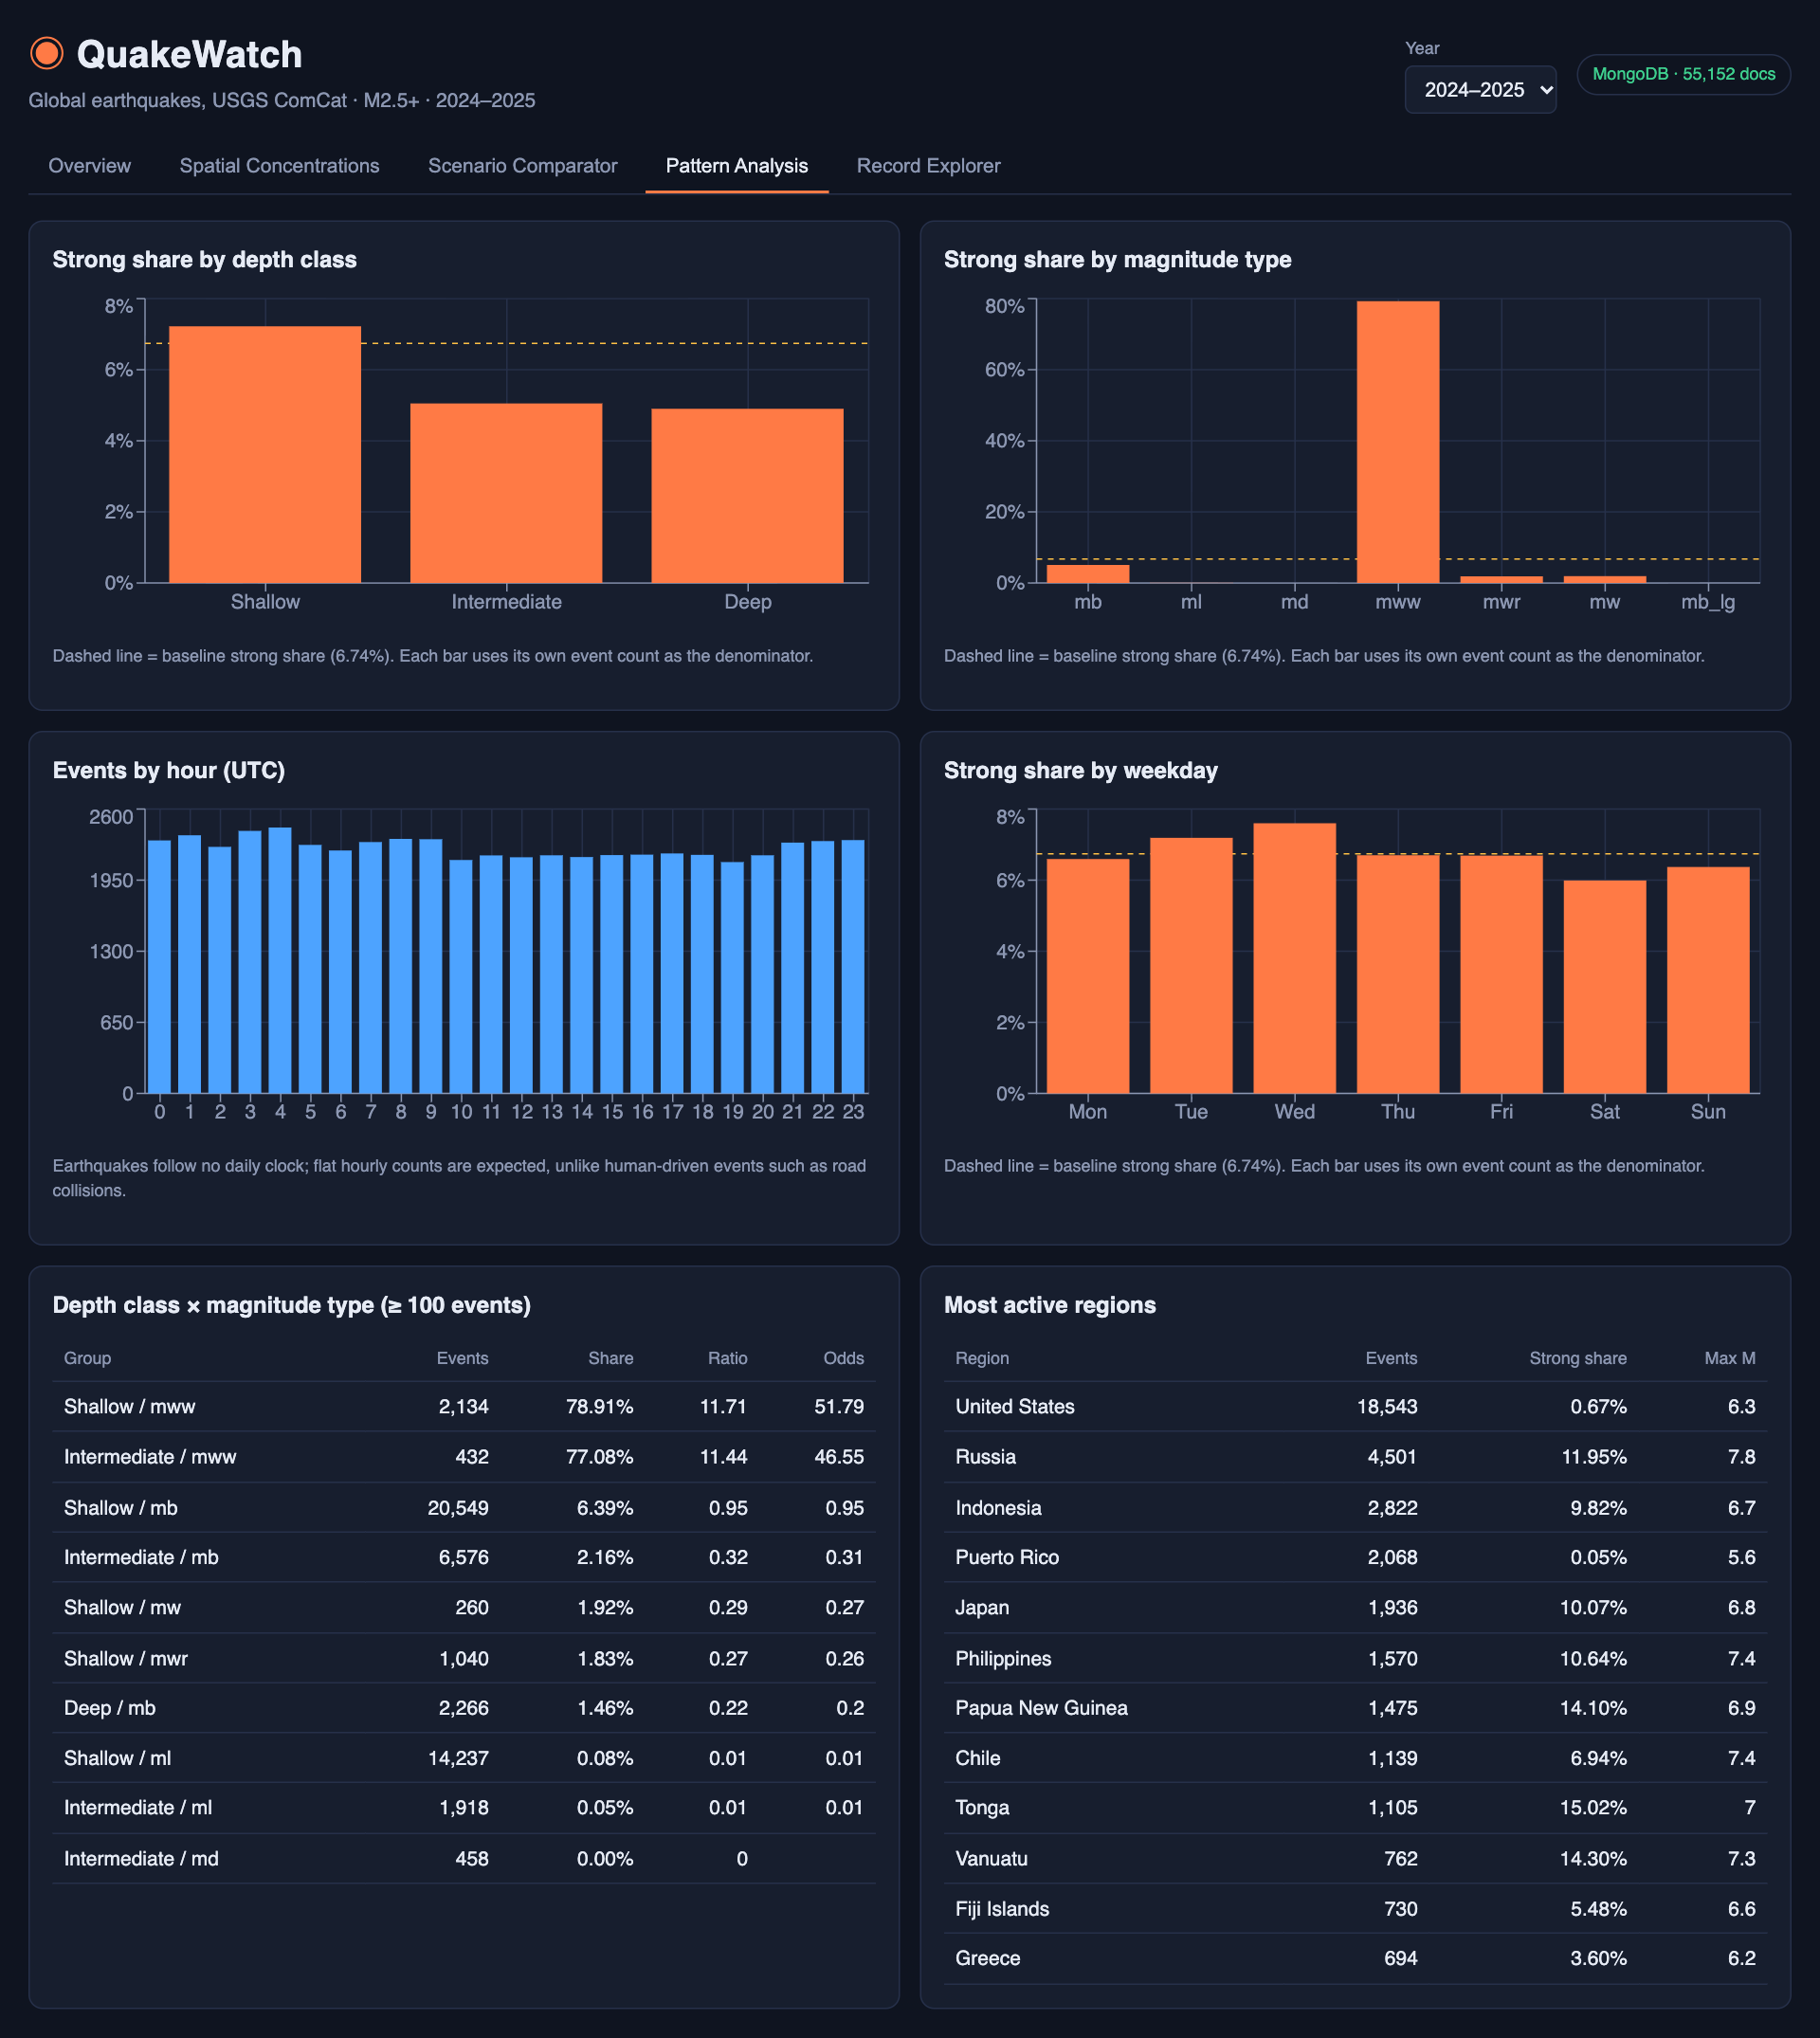
\includegraphics[width=0.85\linewidth,height=0.62\textheight,keepaspectratio]{figures/app_patterns.png}\caption{Actual Pattern Analysis screen: strong share by depth class and magnitude type, hourly counts, weekday strong share, depth$\times$type combinations and the most active regions.}\end{figure}

\subsection{Record search and inspection}
\fig{app_explorer.png}{0.95}{Actual Record Explorer cropped to its search controls.}
Results are paginated in groups of 25 and can be searched by place or event id. Opening an event retrieves the stored document and runs a geospatial query for events within 150~km and one day.

\fig{app_inspector.png}{0.95}{Actual inspector for event \texttt{us6000qw60}, the M8.8 Kamchatka mainshock, listing nearby events within the following day (including M6.3, M6.1 and M6.0 aftershocks within minutes). A second tab shows the stored JSON document.}

\section{BI Dashboard}
\subsection{Exported tables and their grain}
The export pipeline writes a star schema as CSV files.

\begin{table}[H]\centering
\caption{Dashboard tables verified from the exported CSV files.}
\begin{tabular}{lrl}\toprule
Table & Rows & Grain\\\midrule
\texttt{fact\_earthquakes} & 53,952 & One event\\
\texttt{dim\_calendar} & 731 & One date\\
\texttt{agg\_hotspots\_grid} & 1,382 & Grid cell and year ($\ge5$ events)\\
\texttt{agg\_conditions} & 69 & Condition type, value and year\\
\texttt{agg\_regions} & 274 & Region and year ($\ge5$ events)\\
\texttt{agg\_depth\_mag\_matrix} & 28 & Depth class, magnitude class and year\\\bottomrule
\end{tabular}
\end{table}

The same tables can be loaded into Microsoft Power BI Desktop. The repository includes the DAX measures (event count, strong events, strong share, baseline share, share and odds ratios, total energy and a year-aware grid measure using \texttt{TREATAS}) and step-by-step build instructions. The dashboard shown below is the bundled HTML build produced from the same CSV files with Plotly; it mirrors the three-page layout a Power BI report would use.

\subsection{Overview, time and place, conditions}
\fig{bi_overview.png}{0.95}{Dashboard overview page: 53,952 events, 3,636 strong events, 6.74\% share, M8.8 maximum, monthly lines for 2024 and 2025 and a log-scale magnitude-class chart.}
\begin{figure}[H]\centering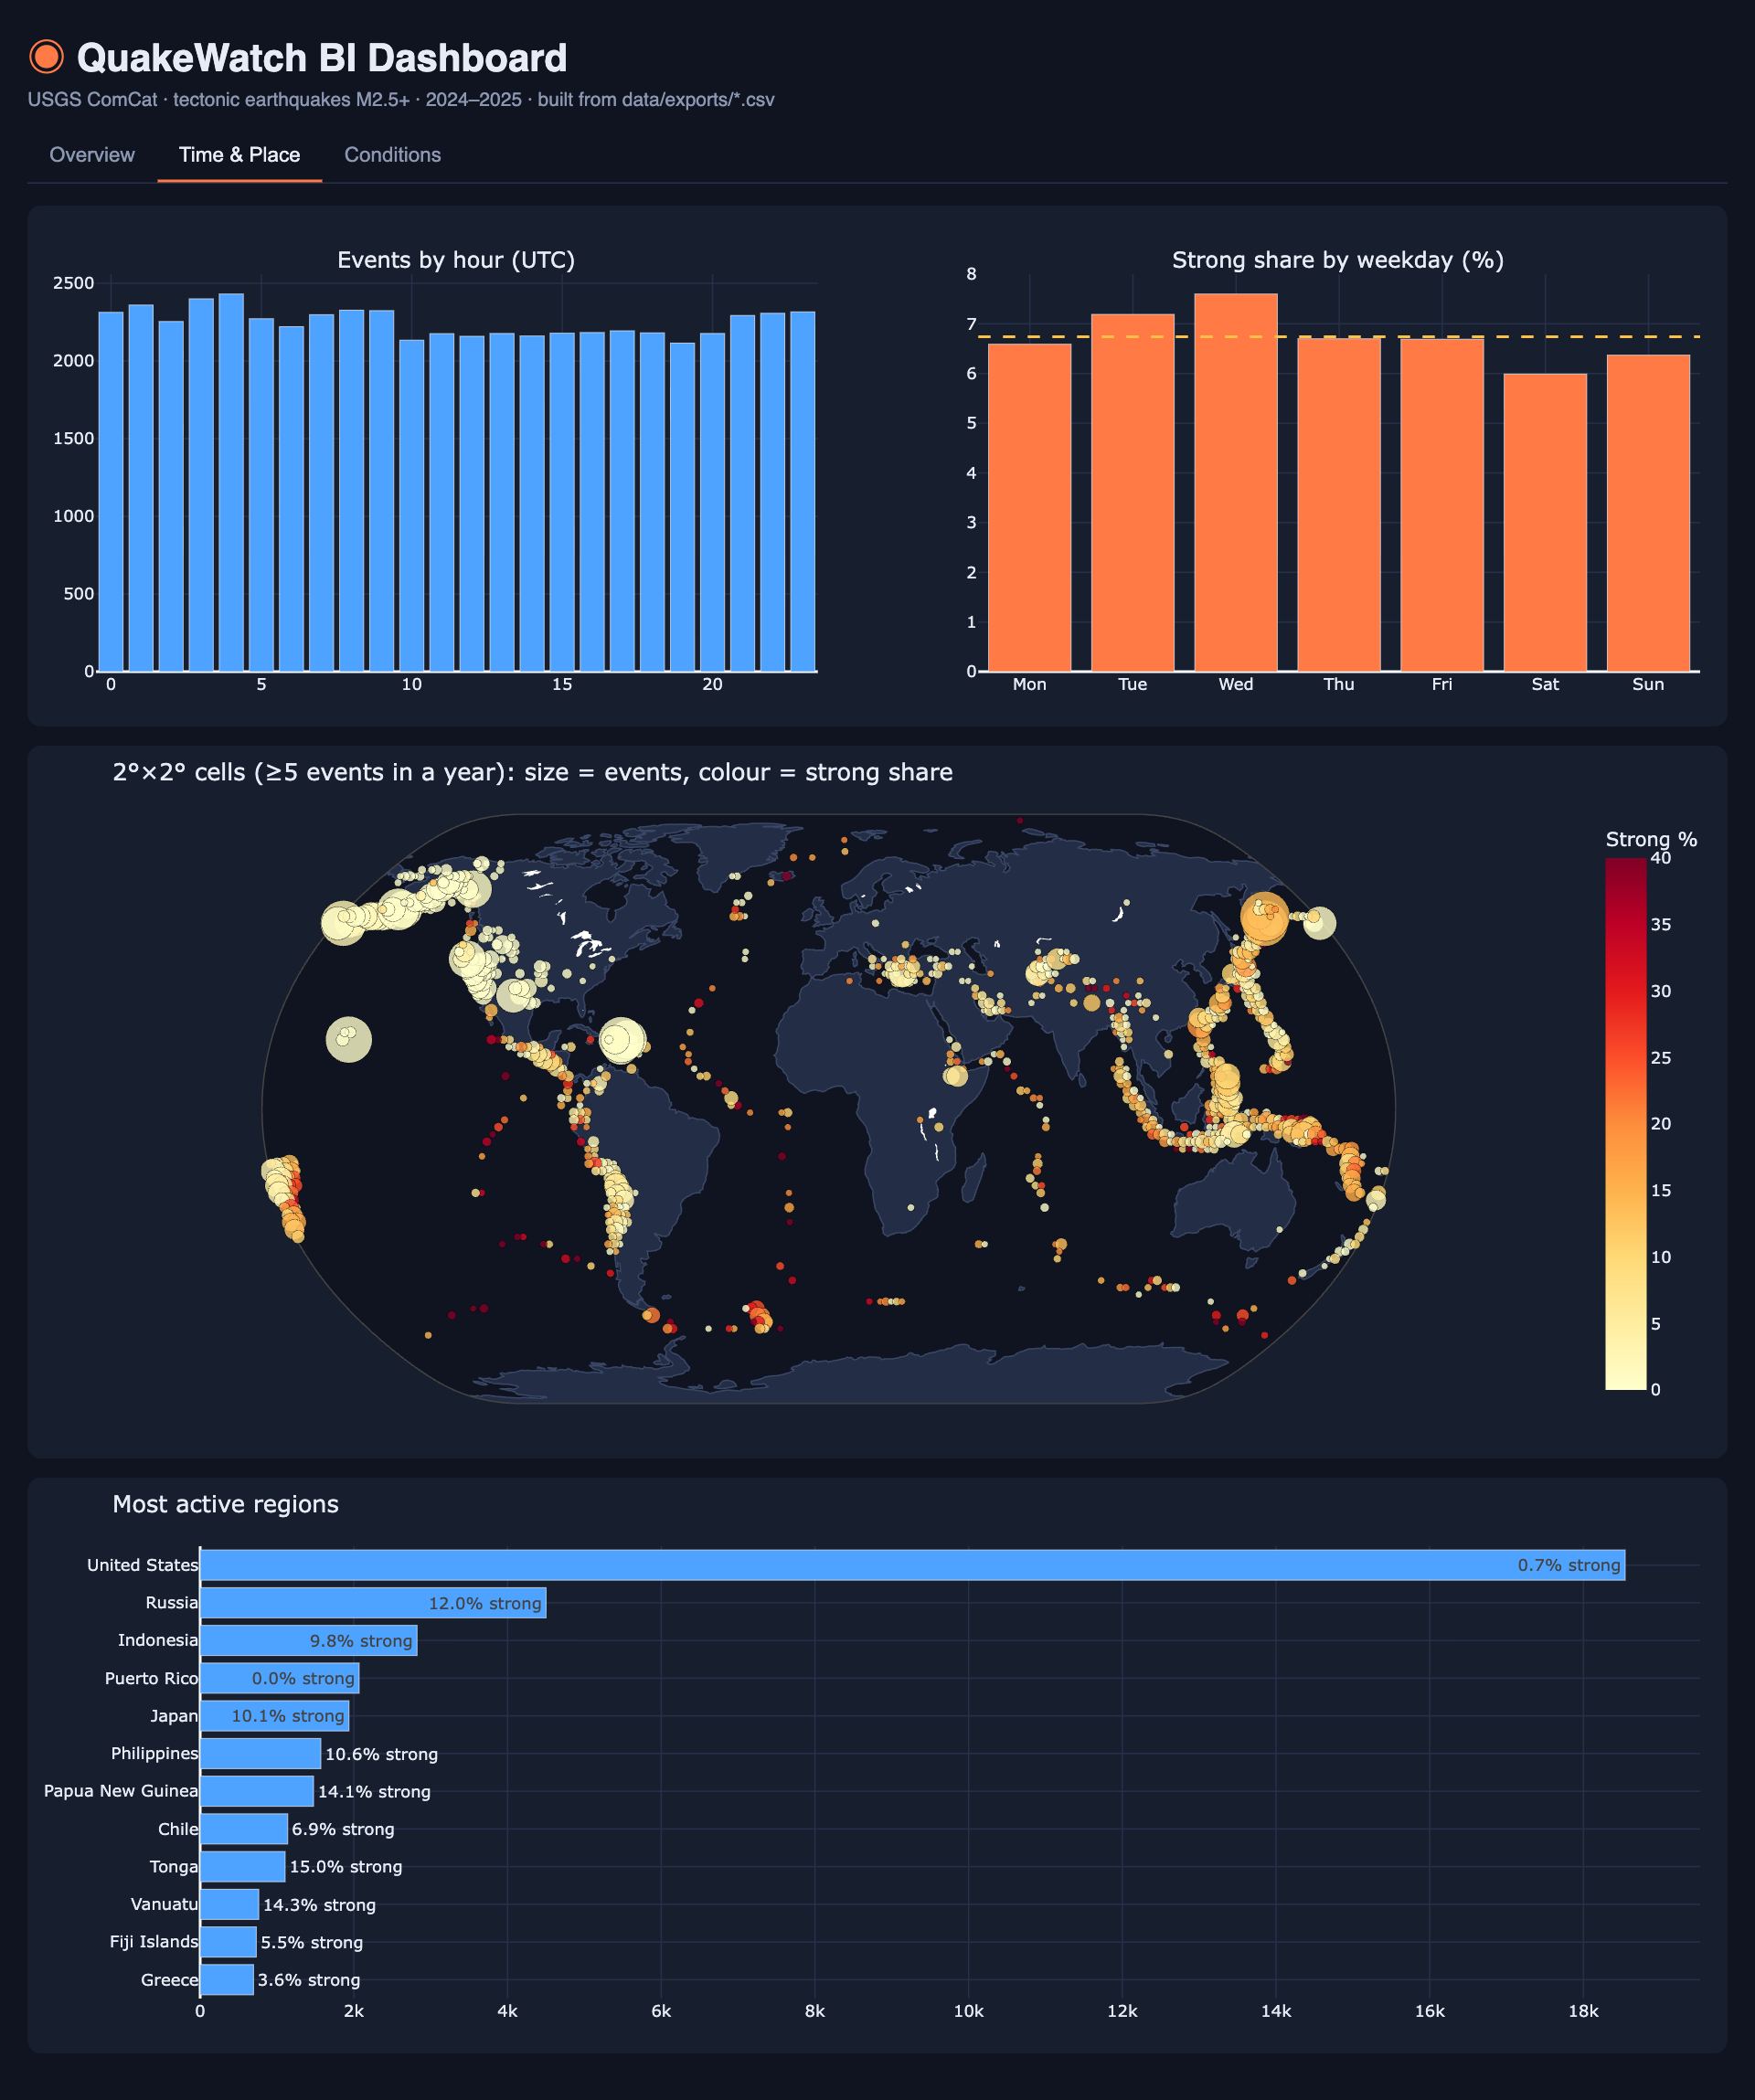
\includegraphics[width=0.85\linewidth,height=0.6\textheight,keepaspectratio]{figures/bi_timeplace.png}\caption{Dashboard time and place page: hourly counts, weekday strong share, a world map of grid cells (size is events, colour is strong share) and the most active regions.}\end{figure}
\begin{figure}[H]\centering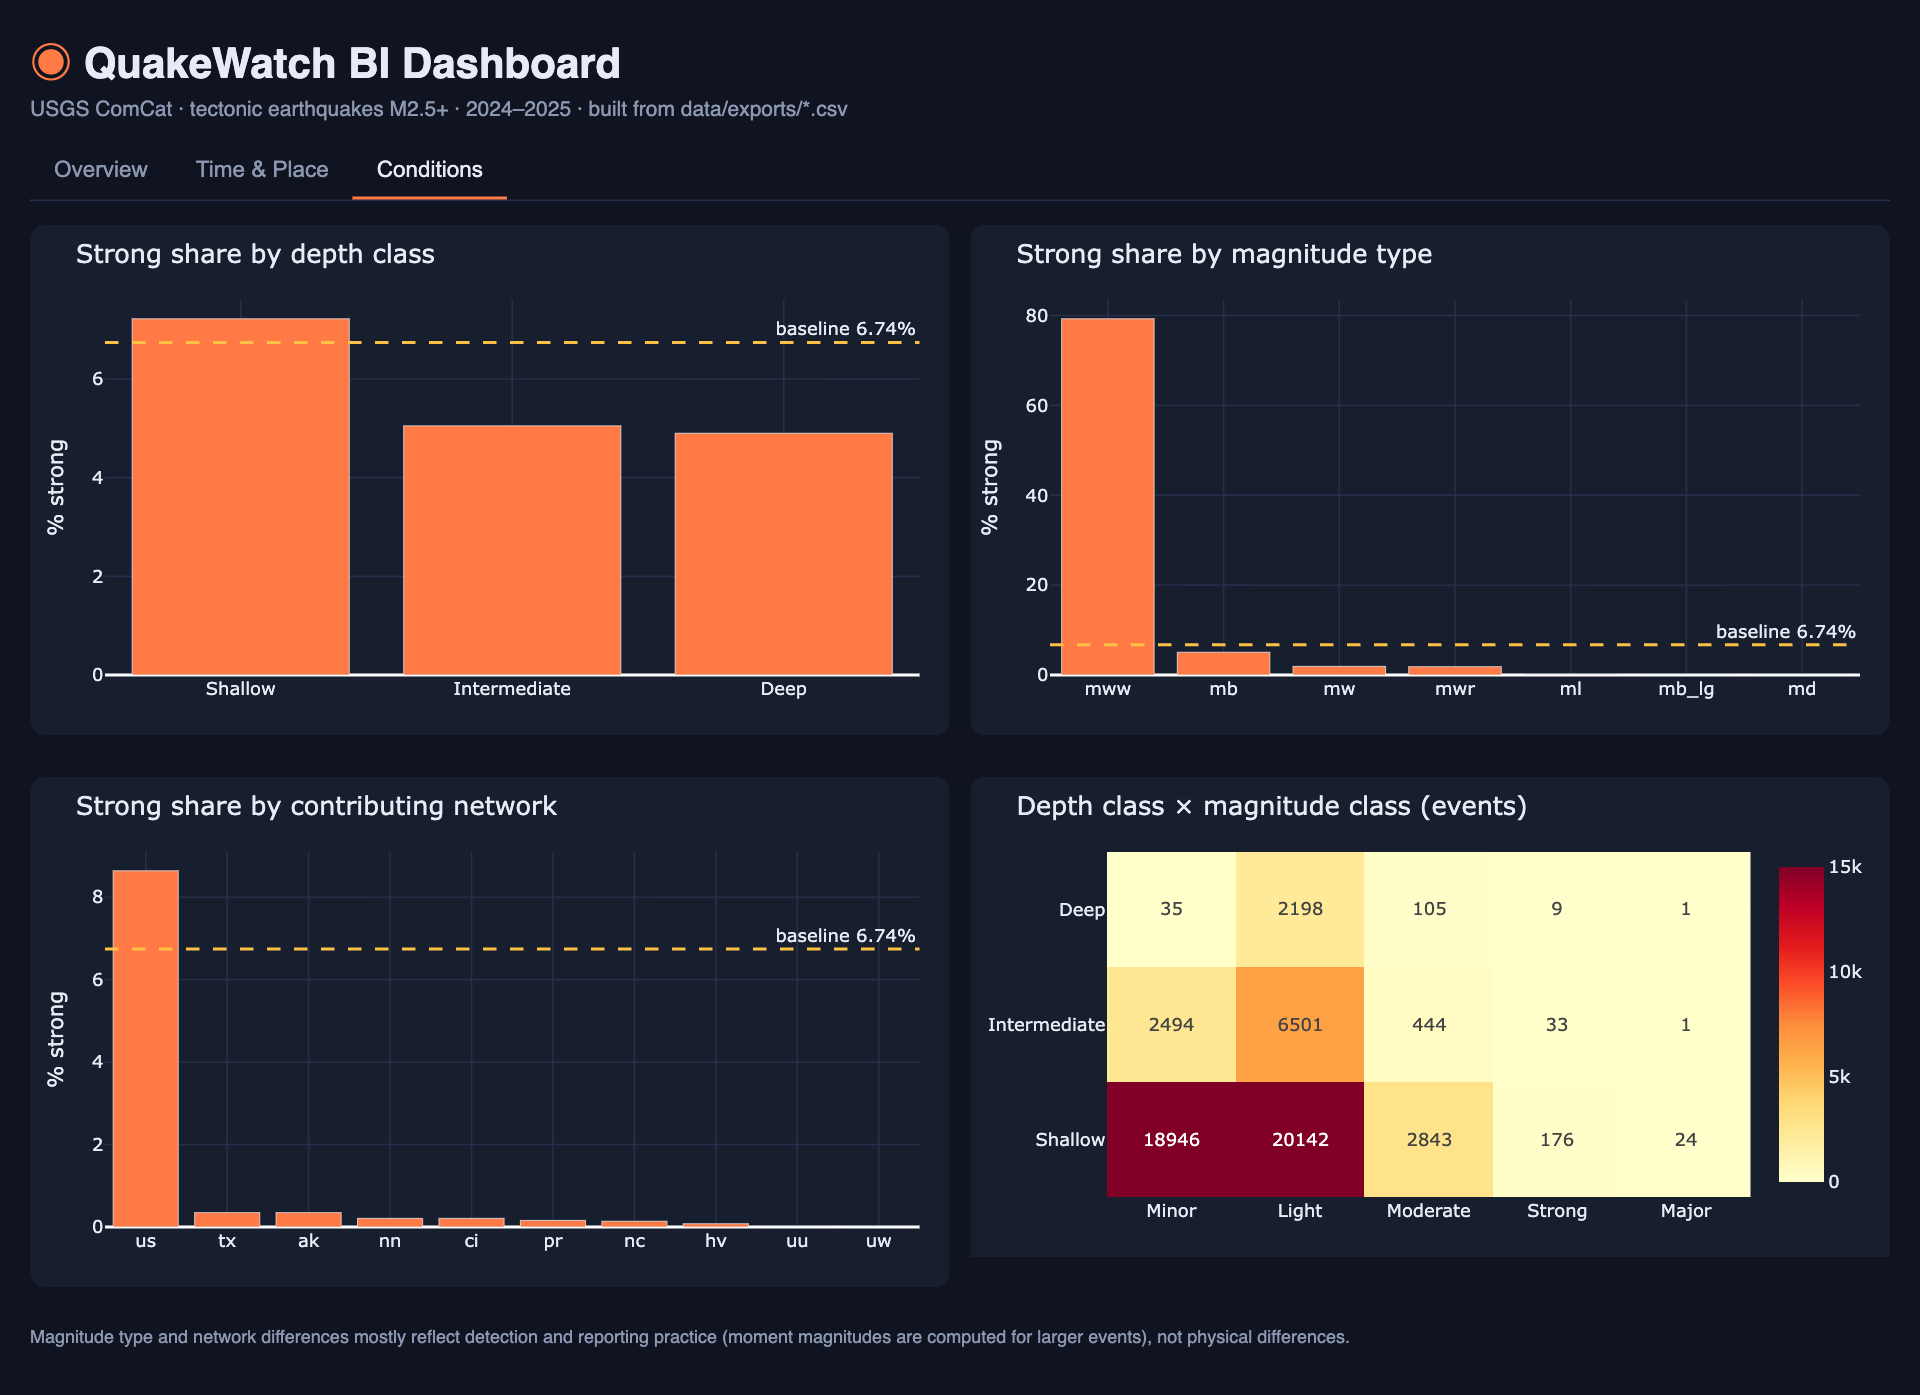
\includegraphics[width=0.85\linewidth,height=0.6\textheight,keepaspectratio]{figures/bi_conditions.png}\caption{Dashboard conditions page: strong share by depth class, magnitude type and contributing network, and a depth-by-magnitude heat map.}\end{figure}

\section{Validation and Limitations}
\subsection{Checks performed for this report}
\begin{table}[H]\centering
\caption{Verification status at report preparation, November 2026.}
\begin{tabularx}{\linewidth}{lX}\toprule
Check & Observed result\\\midrule
Import report & 54,394 raw rows; 442 non-earthquakes excluded; 0 duplicates; 0 invalid coordinates; 53,952 retained.\\
Collection counts & 53,952 + 731 + 469 = 55,152 documents, matching the live database.\\
Severity reconciliation & Strong events 3,636 of 53,952; annual totals sum to the combined totals.\\
Magnitude classes & 21,475 + 28,841 + 3,392 + 218 + 26 = 53,952.\\
API tests & 9 passed (totals, year filter, baseline ratios, temporal sums, combination ratios, pagination, detail and 404).\\
Frontend build & TypeScript check and Vite build completed; a bundle-size warning remains.\\
Screenshots & Distinct web and dashboard pages, visually reviewed.\\
Benchmark evidence & Five timings per query and access path; plan stages retained.\\\bottomrule
\end{tabularx}
\end{table}
Passing tests establishes only what the tests exercise. Report figures were also recomputed independently in Python (pandas) from the raw files and agree with the API and database.

\subsection{Analytical boundaries}
\begin{itemize}
\item \textbf{Catalogue completeness.} Detection thresholds differ by region and network. Counts and strong shares compare reporting practice as much as seismicity.
\item \textbf{Magnitude type.} Strong share by magnitude type reflects when each type is computed, not physics.
\item \textbf{Two years only.} A single M8.8 sequence strongly affects 2025 counts, shares and energy; two years cannot establish trends.
\item \textbf{Region heuristic.} Regions come from parsing the \texttt{place} text; offshore events and unusual strings are only approximately assigned.
\item \textbf{Angular grid.} $2^\circ$ cells are not equal-area, and the map shows at most 400 cells per request.
\item \textbf{Nearby events.} Events within 150~km and one day are candidate aftershocks or foreshocks; no sequence model is fitted.
\item \textbf{Dashboard format.} The BI dashboard shipped is an HTML build; the Power BI model is described by the exported tables and DAX measures, and a \texttt{.pbix} file must be assembled in Power BI Desktop.
\item \textbf{Statistics.} No confidence intervals, completeness-magnitude estimation or hazard modelling are performed.
\end{itemize}

\section{Recommendations and Conclusion}
\subsection{Use of the findings}
Comparisons of strong share should be made within one magnitude type and one catalogue contributor, or restricted to $M\ge4.5$ where the global catalogue is complete. Extending the study to a longer period would separate the Kamchatka sequence from the background rate.

\subsection{Engineering priorities}
\begin{enumerate}
\item Estimate the magnitude of completeness per region and report completeness-adjusted rates.
\item Replace the text-based region heuristic with a gazetteer or tectonic-plate polygons through MongoDB geospatial joins.
\item Add equal-area (for example hexagonal) cells.
\item Identify aftershock sequences with a declustering algorithm instead of a fixed window.
\item Assemble and publish the Power BI \texttt{.pbix} with the provided measures and add a scheduled refresh from the USGS service.
\end{enumerate}

\subsection{Conclusion}
QuakeWatch demonstrates a path from a public earthquake catalogue to a queryable document database, an interactive web application and a BI dashboard. The verified data contains 53,952 earthquakes with a strong share of 6.74\%. The analysis separates frequency from magnitude and from energy, exposes how reporting practice shapes apparent patterns, and shows a single M8.8 sequence dominating 2025. Profiling demonstrates that indexes, including the 2dsphere index with a bounded geographic predicate, cut the documents examined by one to four orders of magnitude. The limitations above define the boundary within which the findings can be presented.

\begin{thebibliography}{9}
\bibitem{usgs} U.S. Geological Survey. \emph{ComCat / FDSN Event Web Service}. Earthquake Hazards Program. Accessed 1 November 2026. \url{https://earthquake.usgs.gov/fdsnws/event/1/}
\bibitem{mongoexplain} MongoDB. \emph{Explain Results}. Execution statistics and query-plan stages. \url{https://www.mongodb.com/docs/manual/reference/explain-results/}
\bibitem{mongo2dsphere} MongoDB. \emph{2dsphere Indexes}. Geographic query support and GeoJSON indexing. \url{https://www.mongodb.com/docs/manual/core/indexes/index-types/geospatial/2dsphere/}
\bibitem{gr56} B.~Gutenberg and C.~F.~Richter. Magnitude and energy of earthquakes. \emph{Annali di Geofisica}, 9:1--15, 1956.
\bibitem{aki65} K.~Aki. Maximum likelihood estimate of $b$ in the formula $\log N = a - bM$ and its confidence limits. \emph{Bulletin of the Earthquake Research Institute, University of Tokyo}, 43:237--239, 1965.
\end{thebibliography}
\end{document}
